\chapter{Approach}\label{sec:approach}

We will now present our contribution and practical approach to build a database
of fingerprints and to capture and identify video traffic of an unaware user
over a compromised network.

We have built a system capable of manipulating the incoming bandwidth of a
network interface, able to obtain fingerprints for a limited number of Netflix
titles at various enforced bandwidth levels, and reconstructed each video's
bitrate ladder. We compare our reconstructed bitrate ladders with the bitrate
ladders constructed from HTTP header (HARs), and report, for each one its the
RMSE.  Eventually, we evaluate the robustness of the saved fingerprints, by
feeding to our identification mechanism, several test-captures of video IDs
(present in our fingerprint's database), at \emph{unseen} bandwidth levels. In
this phase we study the impact of tuning the parameters of the system in
relation to the number of successfully/unsuccessfully identified videos, and
report relevant statistics of each test.

\section{Attack Scenario}

Our own version of the attack, conversely to the one depicted in
\Cref{fig:schema}, does not include the ISP as a potential adversary, nor does
involve an attacker that has compromised an ISP CDN.  We consider a specific
case in which the attacker is a malicious user \emph{i}, with access to the
same network an honest client is using to stream a Netflix title. Attacker
\emph{i} has:

\begin{itemize}
    \item either installed a passive TAP device on a LAN
    \item or gained control of the main switch of a LAN
    \item or compromised an AP over a public WiFi network.
\end{itemize}

For each of the aforementioned scenarios, the steps required for the attacker
\emph{i} to identify video traffic of another user, are the same: the first
phase consists of recording fingerprints of each Netflix title, process them,
store them in a persisent (and convenient for search and retrieval) data
structure, while the second phase consists of exploiting the compromise device
in the network to capture user's traffic and identify the content of the stream
by querying the database of fingerprint.

\section{Video Fingerprinting}

Let $T$ be the set of Netflix titles for Switzerland, we refer to $n$ as the
cardinality $|T|$, which is roughly 3500; consider now the set $R$ as the set of
bandwidth levels shown in \Cref{tab:bandwidths}, we refer to $i$ as the
cardinality $|R|$.

Consider now the cartesian product $T \times R$:

\begin{equation*}
T \times R = \{(t_1, r_1), (t_1, r_2) \dots (t_n, r_i)\} 
\end{equation*}

and its cardinality:

\begin{equation*}
|T \times R| = |T| \cdot |R| = n \cdot i \approx 45500
\end{equation*}

Due to time restrictions, we have decided to fix the size of the set $T$ of
titles to 100, in order to give a proof of concept on the feasibility of such
an attack.  According \cite{netflix-real-time}, we have also decided to bound
the time of each video capture to 4 minutes of playback, as it has been shown
to be sufficient in order to uniquely identify a video over more than 40000
titles.

\subsection{Implementation overview}

We have implemented a set of Python scripts to be able to:

\begin{enumerate}
    \item Crawl the swiss Netflix catalogue to obtain a list of video IDs.
    \item Manipulate the incoming bandwidth of an ethernet network interface.
    \item Invoke \texttt{tcpdump} listening on the same network interface.
    \item Instrument the browser to:
        \begin{enumerate}
            \item Navigate to a specific title URL (identified by the title ID).
            \item Control the Netflix video player by injecting JavaScript code.
            \item Capture HAR metadata via a proxy.
        \end{enumerate}
\end{enumerate}

Note that contrary to \cite{netflix-real-time}, in this phase we do not make
use of adudump, instead, to record traffic, we use tcpdump \cite{libpcap}. The
main reason behind this choice, is the fact that adudump has been conceived to
reconstruct data segments sizes in an online fashion. By doing so, the time
spent by adudump processing each segment, creates an overhead that in turn,
results in noisy measurements.  Adudump can work in an offline-fashion, simply
by passing as input a \texttt{pcap} \cite{libpcap} file, that gets generated
when invoking tcpdump.  We have tested and analyzed this behaviour and visual
evidence is presented in \Cref{fig:online_vs_offline}.

\todo{add plots of adudump's behaviour when invoked online vs on a .pcap file}

\subsection{Crawler}

The script responsible of crawling the Netflix catalogue is
\texttt{crawler.py}.  We use the \texttt{scrapy} Python library \cite{scrapy}
to get a list of Netflix titles divided by genre. Note that, for the sake of
simplicity, we have decided to work only with movies, as for TV series, we
would have need to add checks due to the autoplay function of subsequent
episodes in the viewing phase.

The resulting output of the script is a CSV file with the following structure:

\begin{adu}[caption={Sample of crawled movies}, label={lst:crawl_output}]
ID        GENRE             TITLE

70115629, Family Animation, Despicable Me
70264803, Family Animation, Despicable Me 2
80096067, Family Animation, Ice Age: Collision Course
70220028, Family Animation, Hotel Transylvania
80121840, Family Animation, The Emoji Movie
70021636, Family Animation, Madagascar
70216224, Family Animation, Madagascar 3: Europe's Most Wanted
70213513, Family Animation, Brave
14607635, Family Animation, Mulan
\end{adu}

Due to the fact that a movie can be labeled in more than one category, the
resulting CSV have been filtered to include just one occurrence of each title.

\begin{bash_script}[caption={Command to filter out unique IDs}, label={titles}]
cat netflix_titles/titles.csv | cut -d , -f1 | sort | uniq
\end{bash_script}

\newpage
\subsection{Bandwidth Manipulation}

In order to be able to manually control the bandwidth of the ethernet
interface, we use \texttt{tcconfig} \cite{tcconfig}, a Python wrapper for the
\texttt{tc} \cite{tc} Unix utility to configure traffic control in the kernel.

The script that throttles the bandwidth is \texttt{bandwidth\_manipulator.py},
that invokes the command:

\begin{bash_script}[caption={Enforce a bandwidth rate on the specified interface}, label={tcconfig}]
tcset --device <network_interface> --direction incoming --rate <bandwidth_rate>
\end{bash_script}

\subsection{Tcpdump}

The script that records the capture traffic is \texttt{capture.py}, it calls
tcpdump as below:

\begin{bash_script}[caption={Listens for TCP/IP traffic on the specified
    interface}, label={tcpdump}]
tcpdump -i <network_interface> net 45 -w <output_file>
\end{bash_script}

Note the usage of argument \texttt{net 45}. As Netflix OCAs IP addresses are of
the form \texttt{45.XXX.XXX.XXX}, to simplify the process of identifying
traffic from Netflix, we just use this regular expression for convenience.
Steps required to carry out a more general way to achieve this have been
described in \Cref{dns}.

\subsection{Automated streaming with Selenium}

In order to instrument the browser to automatically stream each title, we have
developed a script that uses the \texttt{Selenium} library \cite{selenium}.
Selenium provides a \texttt{WebDriver} interface capable of controlling various
browsers such as Chrome, Opera, Safari, Firefox and others. One must use the
appropriate version of the WebDriver, according to the browser of choice and
its version. For convenience of use, and support, we have chosen to work with
GoogleChrome and its ChromeDriver interface.

In order to asses the quality of adudump's inference of video segment sizes, we
compare the recorded traffic with HAR \cite{har} metadata. The format of each
HAR file is a json object containing content and session data acquired by the
browser during the playback of the video. For this task, we use
\texttt{Browsermob} \cite{browsermob}, a webproxy built to work with Selenium.

Furthermore, to speedup the capture of each video, we have installed an
extension that is able to control HTML5 video speed playback.

\newpage
We have implemented a class \texttt{netflix\_browser.py} capable of:

\begin{enumerate}
    \item Log in the user to its Netflix account
    \item Navigate to a video url given a video ID
    \item Start the proxy to record HAR metadata
    \item Seek the video to 240 seconds (4 minutes) (avoiding entry credits)
    \item Wait until the buffer of the video reaches 8 minutes (start at 240
        seconds, ends at 480).
    \item Stop the proxy and save the resulting HAR file
\end{enumerate}


\section{Post-processing}

The script that handles post-processing of \texttt{.pcap} output files is
\texttt{post\_process.sh}. It is composed by three main functions.

The first one invokes adudump on the traces recorded with tcpdump, after that,
it extracts the DNSs contained in the HAR metadata and performs a DNS lookup
using Unix's \texttt{host} command. This step is required to get the complete
list of IP addresses of the OCAs that served the video, so that we can filter
all non-video traffic that tcpdump has captured. In addition we threshold ADUs
which sizes are less than 100 kilobytes, as mentioned in \Cref{dns}.

The second function is responsible for generating the bitrate ladders of each
title, and to save all fingerprints in a text file. Given a trace at a
particular bandwidth level $b$, we compute the average bitrate as:

\begin{equation*}
    AVG_{bitrate} = \dfrac{8}{4} \cdot \dfrac{\Sigma_{i=0}^{n} \hspace{2pt} adu_i}{n}
\end{equation*}

We average over all ADUs (sizes are in bytes), divide by 4 seconds (approximate
lenght of a video segment according to \cite{netflix-real-time}), and multiply
by 8 to get a measure in \emph{bits/s}. 

We repeat the process decribed above, also by generating fingerprints from the
HAR records we capture with our proxy. By doing so, we can reconstruct the
\emph{true} bitrate ladders, for each capture, and use them as a term of
comparison to asses the quality of the ADU's reconstruced ladders. For each
ADU reconstructed bitrate ladder, we compute the \emph{mean-normalized} RMSE
with the HAR reconstructed ones as shown in \Cref{sec:rmse}.

\begin{figure}[!h]
  \centering
  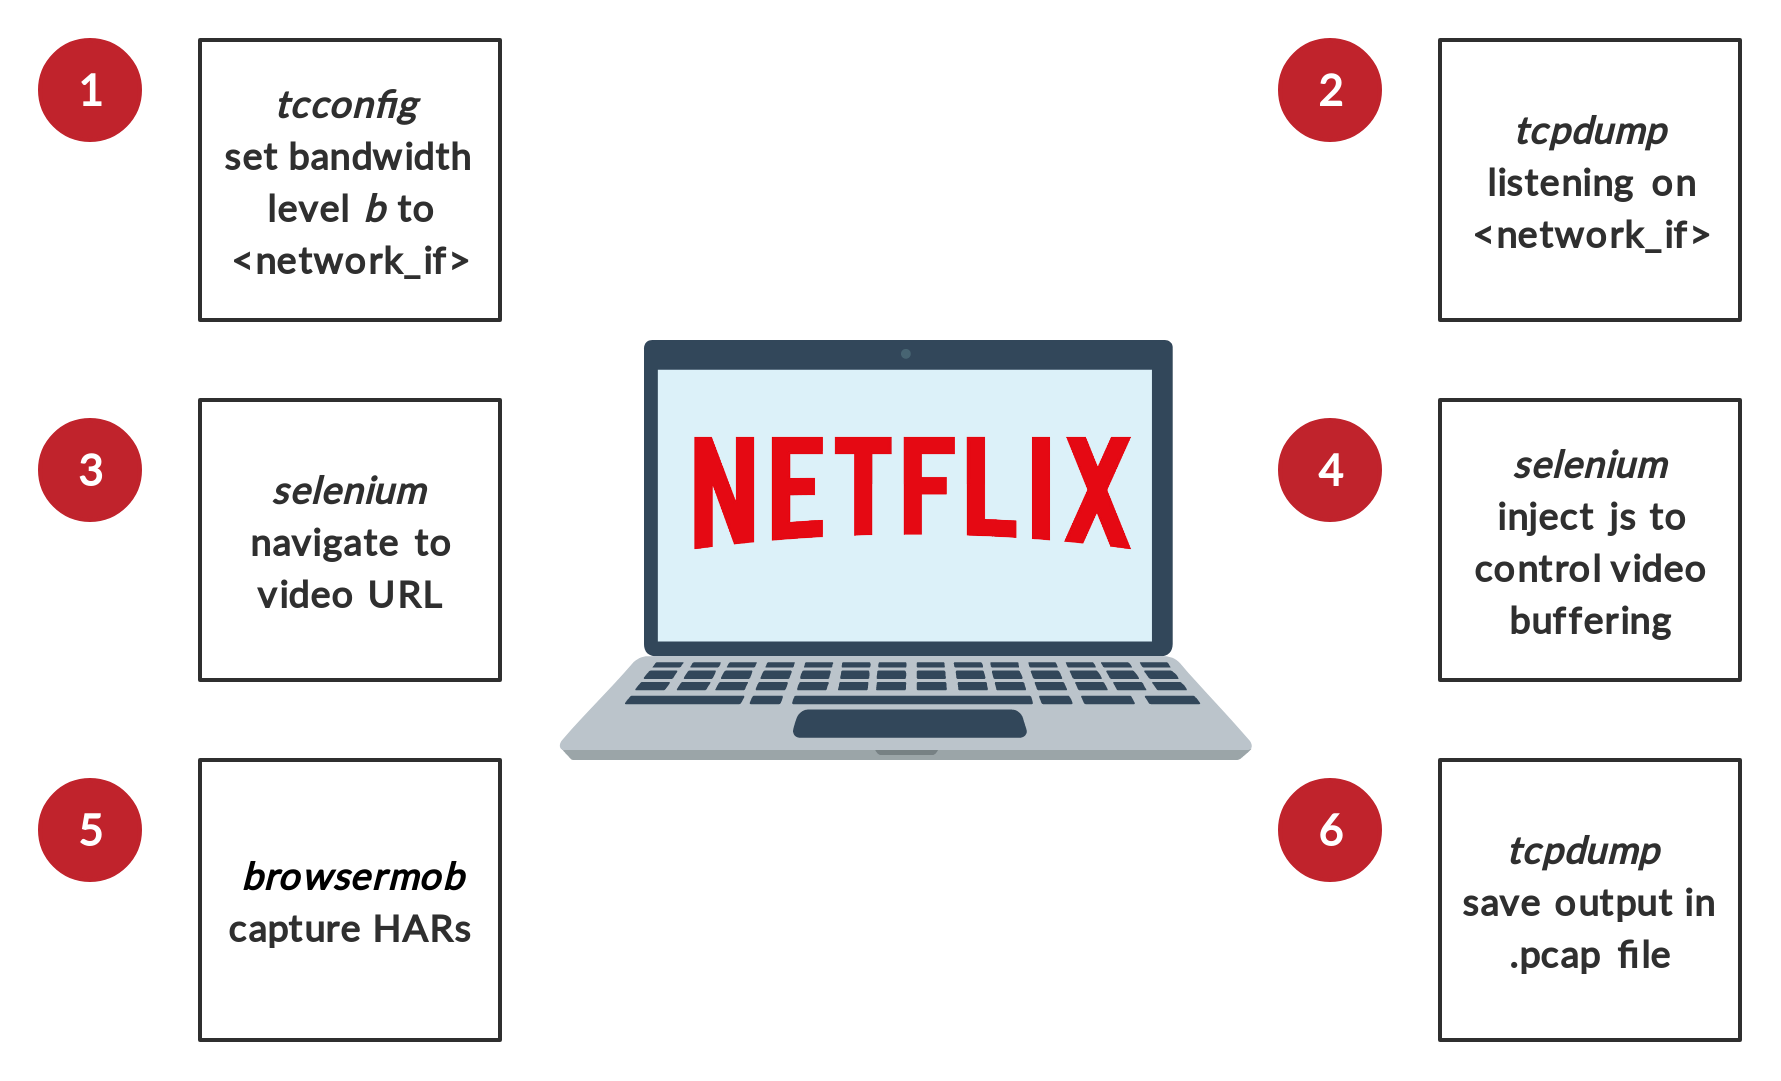
\includegraphics[width=\columnwidth]{img/fingerprints.png}
  \caption{Overview of the process of acquiring video fingeprints.}
  \label{fig:fingerprints}
\end{figure}


\section{Capturing video traffic}

In order to evaluate the attack, we capture a set of video traffic traces (the
ones the attacker $i$ can retrieve by mirroring traffic on the compromised
device), at unseen enforced bandwidths. In practice, our database of
fingerprints hosts 100 movie titles at the 13 bandwidth levels presented in
\Cref{tab:bandwidths}, while the new \emph{unseen} bandwidths are listed below
in \Cref{tab:unseen_bandwidths}.

\begin{table}[htb]
  \centering
  \begin{tabular}{|c|c|c|c|c|c|c|c|}
    \hline
    \multicolumn{8}{|c|}{\textbf{Unseen Bandwidth levels (Mbps)}} \\
    \hline
    0.5 & 1.0 & 3.0 & 5.0 & 6.0 & 8.0 & 12.0 & 18.0 \\
    \hline
  \end{tabular}
  \caption{Enforced unseen bandwidth levels.}
  \label{tab:unseen_bandwidths}
\end{table}

As for the acquisition of fingerprints, we repeat the same exact steps to build
our testing set, that is composed by the same 100 titles recorded at the new 8
unseen bandwidth levels depicted above. 

\newpage
\section{Identification}

For this purpose, we have implemented a modified version of the search tree
used in \cite{netflix-real-time}. All the scripts in this Section can be fuond
under the \texttt{identify} directory located at the root of the project.

The identification process involves two parties: a Java program that runs as
a proxy to our database, and a Python script that takes as input the
fingerprints of captured traffic to query the database for matches.

The Python script queries the Java process running the KD-tree, that returns a
list of possible matches for the given captured trace.

\begin{figure}[!h]
  \centering
  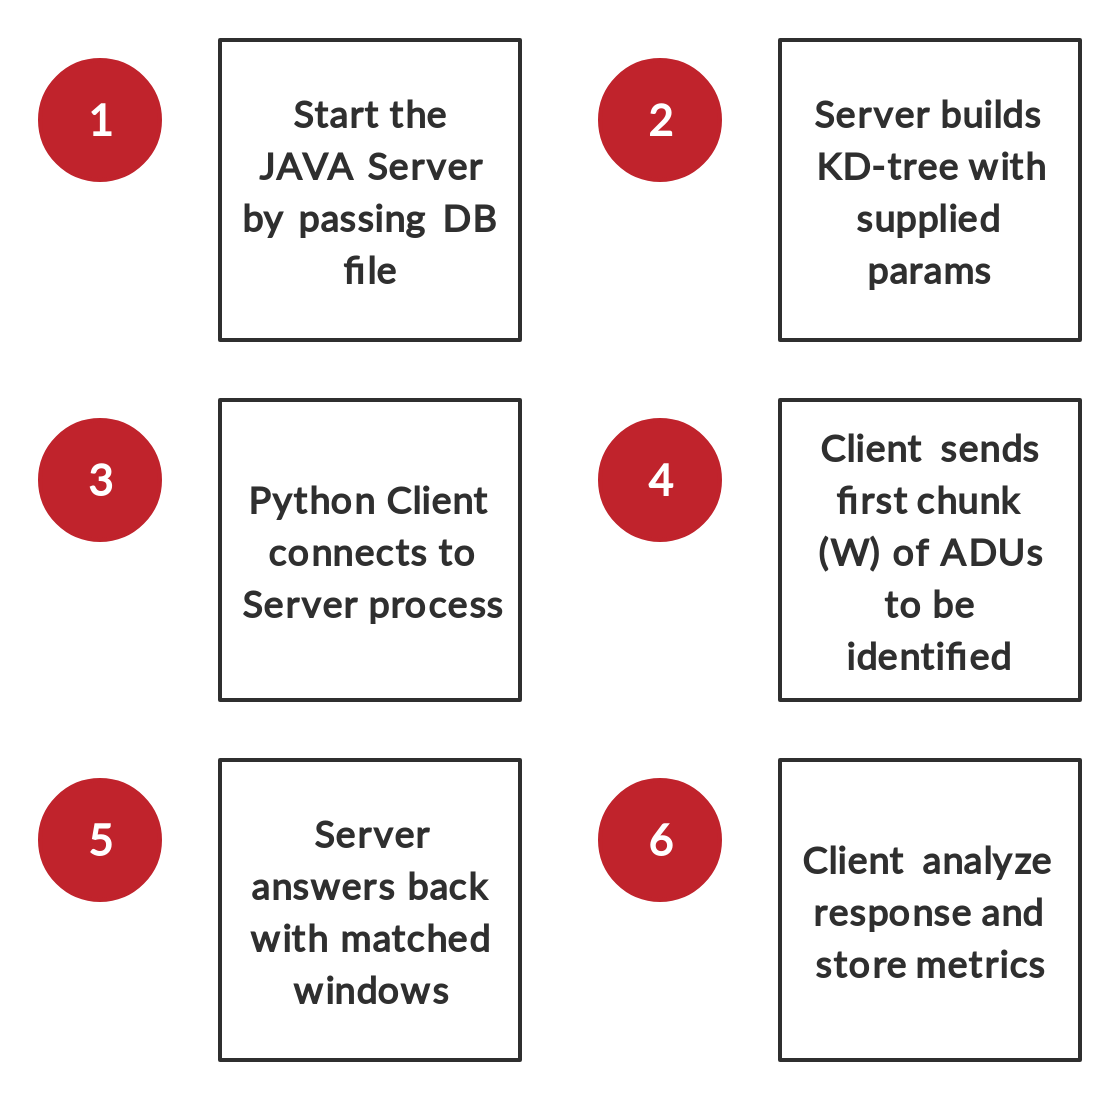
\includegraphics[width=.6\columnwidth]{img/identification.png}
  \caption{Overview of the process of identification.}
  \label{fig:identification}
\end{figure}

\subsection{KD-Tree}

The code that implements the KD-Tree is found under the \texttt{server}
directory. \texttt{runServer.sh} runs an instance of the system and requires 6
parameters as input:

\begin{bash_script}[caption={Start the Java Server}, label={lst:java}]
        cd server && ./runServer.sh <db_file> <capture_file> <window_size> <key_size> <key_mode> <key_delta> <
\end{bash_script}

To simplify writing, we assign to the following parameters a corresponding greek letter:

\begin{itemize}
    \item $\omega$ represents the window size.
    \item $\kappa$ is the key size. 
    \item $\mu$ reprents the key mode.
    \item $\delta$ 
    \item $\rho$ represent the minimum pearson correlation coefficient to accept a match..
\end{itemize}

The above script executes \texttt{Netflid.jar}, composed by the following
Java classes:

\begin{itemize}
    \item \texttt{Netflid}: main Class, sets up the \texttt{KDTree}, and start a
        \texttt{ServerThread} instance.
    \item \texttt{KDTree}: implements the KD-tree data structure.
    \item \texttt{ServerThread}: listens for the client to send data, queries
        the \texttt{KDTree}, and respond to the client with matches.
    \item \texttt{Window}: constructs and store the key to search the \texttt{KDTree}.
    \item \texttt{Movie}: represents a movie instance.

\end{itemize}

\subsection{Building the KD-Tree}

\texttt{Netflid} is the main class that creates a \texttt{KDTree} instance
(with $K$ being the dimension of the search key), to which every record in the
database is added to. Each record, has the following structure:

\begin{bash_script} 
ID              AVG_BITRATE  SEGMENTS
896970_15000    3038         321427,198559,113973 ...
\end{bash_script}

The \texttt{ID} of the record is formed by the video ID, and the
enforced bandwidth at which the title has been captured
(\texttt{896970\_15000}), represents movie ID 896970 \emph {Red Heat},
recorded at 15.0 \emph{Mbps}. Note how the number of segments for each
record is not fixed, as explained in \Cref{sec:problems}.  For each
record, we create an instance of \texttt{Movie}, in which we store its
ID, the average bitrate and its segments. Based on the number of
segments $s$, we build $s-1$ \texttt{Window}s of $\omega$ segments.
For each window, we build a search key of dimension $K$, in one of the
following modes, expressed by $M$: 

In case $M$ \texttt{== 0}, the key gets constructed by assigning the
total sum of the segment sizes in the window as first dimension; the
rest $K - 1$ dimensions, represent the proportion of data received
within $\dfrac{\omega}{K-1}$ segments with respect to the
aforementioned total in the first dimension.

In case $M$ \texttt{== 1}, instead we store the average bitrate
(computed as in \Cref{sec:idk}) of all segments in the window as
first dimension, then each of the $K-1$ dimensions is the average
bitrate of $\dfrac{\omega}{K-1}$ segments, normalized again by the
first dimension.

\subsection{Querying the KD-Tree}

After having added the key to the \texttt{KDTree}, we start a
\texttt{ServerSocket} thread that listens for incoming connections from the
client. \texttt{ServerThread} is the runnable class responsible for consuming
the input of the socket the Python client communicates through. It reads up to
$\omega$ lines, and creates a \texttt{Window} and its corresponding key with
the same method used when adding records from the database to the
\texttt{KDTree}. Then it queries the \texttt{KDTree} by generating an upper,
and a lower range key, with the specified $\delta$ (the greater $\delta$ is,
the broader the search will be). The \texttt{KDTree} then retrieves a list of
matching windows with a \emph{pearson correlation} coefficient bigger than
$\rho$.

